
\subsection{A2 Governance}

The governing authority (a) adopts policies which are consistent with the school’s mission and vision and support the achievement of the schoolwide learner outcomes, i.e., global competencies, (b) delegates implementation of these policies to the professional staff, and (c) monitors results.

\subsubsection{Clear Policies and Procedures}

\indicator{There are clear policies and procedures with regard to the selection, composition, and specific duties of the governing authority.}

\prompt{Evaluate the clarity of the policies and procedures regarding the selection, composition, and specific duties of the governing authority.}

\begin{findings}
The CMIS Board of Directors (the board) has developed clear policies with regard to the selection, composition, and specific duties of the governing authority. 

The board is composed of nine members: four are appointed by the Church of Christ in Thailand (CCT) - our parent organization, three through their role at the school (Director, Manager, Superintendent), one teacher representative, and one parent representative. The teacher representative is elected by the staff and it is preferred (not required) that they serve in a school leadership role (e.g., team leader). They serve for a minimum of two years.

The PTG representative is elected through a process, described further in the \href{http://blogs.cmis.ac.th/ptg/bylaws/}{PTG Bylaws} and serves for a minimum of two years.

Board member roles and responsibilities are clearly outlined and described in the Policies and Procedures Handbook for Administration of the Institutions in the Church of Christ in Thailand

In order to remain current in professional practice, the CMIS Board invited outside consultant John Ritter in September, 2015 to facilitate the discussions on future decisions and outcomes. At this time, the board engaged in a review of its annual goals and the review resulted in a reflection of the school's strengths, weaknesses, threats, and opportunities. 

The board revisited these responsibilities in November 2016 and created a document entitled:  \href{https://docs.google.com/document/d/1EyIeD5g0RDANtZzH5rsCkvDp5ea_bQ2G9rWnhz4QbSc/edit?ts=5881d18d}{Principles of Good Practice}  to better align the board’s responsibilities with the school’s mission, vision, and to further support the achievement of the schoolwide learner outcomes. They also drafted a policy outlining individual board member responsibilities and duties: \href{https://docs.google.com/document/d/14e90Qr4edga9mEZuHIclWeraZ5jgq052IUwcnxTHQZw/edit?ts=5881b471}{Individual Board Member Principles of Good Practice}. These items will be finalized by the board and voted upon for adoption in the February 2017 board meeting.

The board is currently studying the the National Association of International Schools Trustee Handbook (\href{http://www.nais.org/Articles/Pages/NAIS-Trustee-Handbook-Resources.aspx}{NAIS}) together, and using it as a reference for creating future board development.

The board is currently creating a CMIS Board Handbook which is scheduled for compilation by September 2017. This initial version will used as a reference tool for future policies and procedures with regard to the selection, composition, and specific duties of the governing authority. 

\minor{So what...}

The board has focused strongly on adopting policies which are consistent with the school’s mission, vision, and support the achievement of the schoolwide learner outcomes.

Completing the CMIS Board Handbook will allow the BOD to identify additional ways to improve in this area and help to find effective means to communicate these out to our community.
\end{findings}

\subsubsection{Pretraining of Potential Board Members}

\indicator{Individuals who seek board membership or are being considered as appointees by the board will have some form of training in the principles and skills essential to the effectiveness of the school board.}

\prompt{Evaluate the effectiveness of the training that is offered to prospective or new school board members.}

\begin{findings}
CMIS became an official member of the \href{http://www.nais.org/Articles/Pages/NAIS-Trustee-Handbook-Resources.aspx}{National Association of Independent Schools} in 2016 in order to access the most recent research and trends on school governance. 

New CMIS Board members are given a copy of the “International Trustee Handbook of School Board Leaders” to prepare them for their initial tasks of being a CMIS Board member. 

Currently, the CMIS Board utilizes an informal mentoring system where new board members are provided insight and guidance through informal discussions from other senior board members. 

The board chair and newly appointed Superintendent are currently completing book studies together of \textit{Living From the Heart Jesus Gave You} and textit{Joy Starts Here}.Their studies review the Christian ethos, how it relates their own personal journey in Christianity and the Christian vision for CMIS. This mentorship relationship highlights the importance of a strong partnership between the chair and the head of the school,

``It is critical that the chair and head make every effort to establish a solid and mutually supportive relationship based on respect and trust, develop the capacity to be forthright and candid, and listen to and learn from each other's feedback. The board chair and the head share the same goal: providing effective leadership for the school.'' \textit{NAIS Trustee Handbook} p.125

Current and prospective board members have attended EARCOS workshops together for the past two years. Sessions attended by board member at the 2015 EARCOS Leadership Conferences:
\begin{itemize}
\item Learning from Lincoln Leadership
\item Strategic Planning for Effective School Boards 
\item Parent Teacher Organizations: Effective Communication
\item Effective Adoption and Resource Cycles 
\end{itemize}

All board members were asked to review and sign \href{https://docs.google.com/a/cmis.ac.th/document/d/1sVjFjeVtwbk0-n8GsM5K_XzZSn2wejtlJ3kurXUrKGU/edit?usp=sharing}{CMIS Board of Directors: Roles and Responsibilities} of the \href{https://docs.google.com/a/cmis.ac.th/document/d/1sVjFjeVtwbk0-n8GsM5K_XzZSn2wejtlJ3kurXUrKGU/edit?usp=sharing}{Board and CMIS BOD Code of Conduct} at the beginning of the 2016-2017 school year.

\minor{So what...}

The CMIS Board of Directors has worked hard to increase the pre-training and support for new board members but acknowledges that it can do more. The CMIS Board Handbook will include further strategies for new BOD training and support.
\end{findings}

{\centering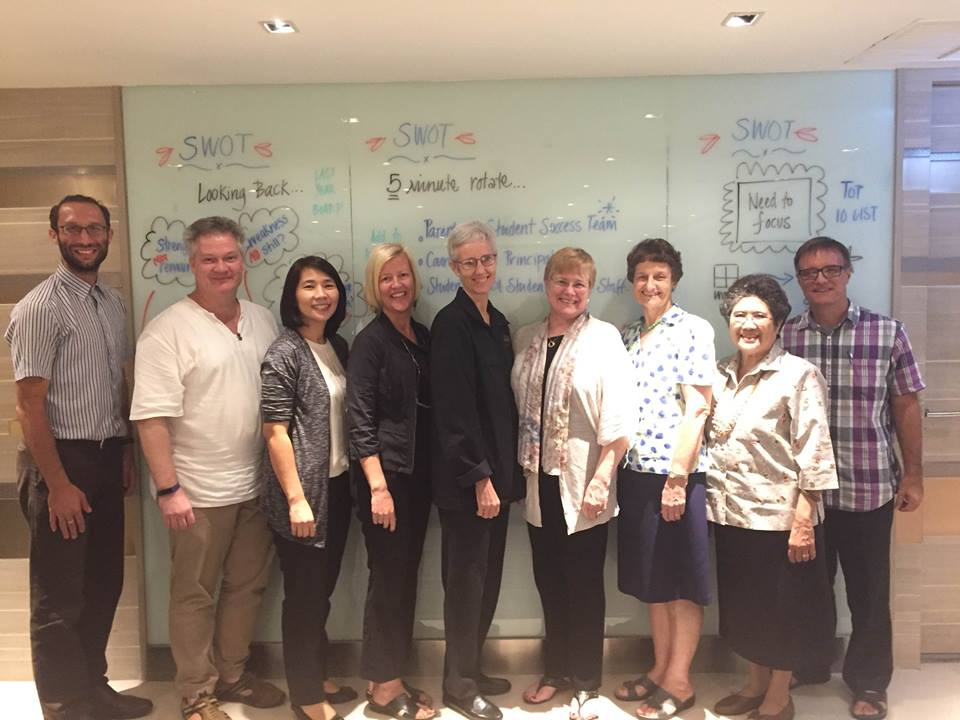
\includegraphics[width=\textwidth]{chapter4_A2.jpg}}

\subsubsection{Relationship of Policies}

\indicator{The governing authority’s policies are directly connected to the school’s vision, mission and schoolwide learner outcomes that focus on student achievement of global competencies.}

\prompt{Evaluate the adequacy of the policies to support the school’s vision, mission, and schoolwide learner outcomes through its programs and operations.}

\begin{findings}
The CMIS Board models collaborative leadership that provides a unified direction to all leaders and members of the staff. This direction is clearly connected to the school’s purpose evident in its vision, mission, and \href{https://docs.google.com/document/d/1bIbV9pgGz2vpXYJdnRzL_Od5PS35egy7lgBOBuszgD4/edit}{student learner outcomes} (SLOs).

The effective involvement of all stakeholders, starting from the governing authority, in formulating and implementing the vision, mission, and SLOs, ensures that student achievement is the focus of all school decisions. The guidance and leadership of the governing authority provide the momentum necessary to effectively address our vision, mission, and SLOs.

The CMIS Board is responsible for providing the necessary learning programs and operations that support CMIS curriculum and resources, attracting and retaining quality employees, and ensuring the availability of learning materials and supplies. Through the budget funding process, the board also supports professional development for teachers, administrators, support staff, and the board.

At a summer 2016 Board Retreat, the current CMIS Board created a plan for areas of improvement that are based on the following topics: 

\begin{itemize}
\item Stakeholder communications
\item Funds development
\item Strategic planning
\item board handbook
\end{itemize}

The board also developed strategies and procedures to address these areas and are in the process of developing measurable goals to evaluate the effectiveness of these actions. The goals focus on the board’s responsibility to be good stewards of its resources, its fiduciary responsibilities, and on providing clear, strategic leadership to ensure CMIS is viable for years to come.

The CMIS mission, vision, and SLO are consistently integrated into the board agenda template. This is done to ground the meeting in the important work of school outcomes and focus members on our students and their achievement. 

\minor{So what}

CMIS acknowledges that the past decisions and proposals of the board have often been recorded in board minutes that can be difficult to locate and refine. This limits the current board’s ability to effectively evaluate the connectedness of CMIS Board practices, in relation to the the school’s vision and mission.

In an effort to address this challenge, the board has appointed a committee to facilitate the creation of a CMIS Board Handbook, which is scheduled for compilation by September 2017. This Handbook will make it easier for evaluation as the policies will be created in a common format and available in a central location. 
\end{findings}

\subsubsection{Involvement of Governing Authority}

\indicator{The governing authority is involved in the regular review and refinement of the school’s vision, mission, and schoolwide learner outcomes. The governing authority uses a variety of strategies to remain current in research-based knowledge about effective schools.}

\prompt{Evaluate the processes for the involvement of the governing board in the regular review and refinement of the school’s vision, mission, and schoolwide learner outcomes.}

\begin{findings}

The governing authority is involved in the regular review and refinement of the school’s \href{http://cmis.ac.th/about/vision}{vision, mission, and schoolwide learner outcomes}. It also uses a variety of strategies to remain current in research-based knowledge about effective schools.

As mandated by the ``Board of Directors Roles and Responsibilities of the Board'', the board reviews the mission, vision, and schoolwide learner outcomes at the beginning of each school year. For example, in May 2014 the board voted to revise the vision and mission statement, and in 2015 voted to revise the schoolwide learner outcomes so they were more measurable and in line with the Focus on Learning recommendations. 

In order to remain current in research based knowledge about effective schools, the CMIS Board invited outside consultant John Ritter in September, 2015 to facilitate board development  that reviewed the characteristics of effective school boards. In summary, the workshop focused on:

\begin{itemize}
\item Having a shared vision about high capabilities of both students and staff
\item Being policy and accountability driven
\item Engaging in goal-setting processes that can drive action in the school to improve
\item Aligning resources around those goals
\item Using data to diagnose problems and to monitor and drive continuous improvement efforts
\item Communicating and engaging with the community
\item Working well together as a team 
\end{itemize}

These characteristics have been used as the foundation for CMIS Board planning and will provide the framework of the CMIS Board Handbook. The board chair also studied the book, \href{https://www.amazon.com/Governance-Leadership-Reframing-Nonprofit-boards/dp/0471684201}{\textit{Governance as Leadership}}  which reviews the process of generative thinking in relation to strategic planning and plans to also use the guidelines from this research based book in the compilation of the CMIS Board Handbook.

CMIS is a member of The International School Association of Thailand (ISAT). ISAT works with government ministries to keep current of the benefits of international education in Thailand and promotes quality international school education.

The quality of education offered at the ISAT member schools has been recognized by accreditation organizations such as the \href{https://en.wikipedia.org/wiki/Western_Association_of_Schools_and_Colleges}{Western Association of Schools and Colleges} (WASC), and the \href{https://en.wikipedia.org/w/index.php?title=Council_of_International_Schools&action=edit&redlink=1}{Council of International Schools} (CIS).

The CMIS Superintendent and Manager serve on the CMIS Board and attend the \href{https://drive.google.com/a/cmis.ac.th/file/d/0Bwny3HLdIIS7LUtqTlR2REhsLVBkWHVib3k3V1hsWVFtUzIw/view?usp=sharing}{ISAT quarterly meetings} together. It is a great opportunity to review the CMIS vision, mission, and schoolwide learner outcomes in relation to other schools in Thailand. 

At the ISAT meetings there are often guest speakers (e.g., in November, Dr. Chaipreuk Sereerak, Permanent Secretary, Ministry of Education and Mr. Krittachai Aroonrat, Secretary General, Office of Private Education Commission) . Their expertise and guidance assist the board in remaining current about effective schools international school policy and educational trends in Thailand (\href{http://www.isat.or.th/members/announcement-updates/minutes-isat-general-member-meeting-22016}{sample minutes}).

CMIS Manager, \href{https://drive.google.com/a/cmis.ac.th/file/d/0Bwo-i12FeO0rY1V1SGtuSzJBd1U/view?usp=sharing}{Patcharin Jingkaojai} was elected in 2016 to the ISAT Management Committee which provides leadership and support to membership schools throughout Thailand. In September 2016 the Management Committee organized the \href{https://drive.google.com/a/cmis.ac.th/file/d/0Bwo-i12FeO0rQ0JOZ09JVTNEUTA/view?usp=sharing}{Regional Member Meeting} that was hosted at CMIS. 

In 2016, the CMIS Superintendent, Nel Capadona joined the ISAT Professional Development Committee and assists with supporting professional development, school development, and networking for ISAT member schools. In November 2016 they promoted the \href{https://drive.google.com/a/cmis.ac.th/file/d/0ByVFfrm0zfolSXFEZFJVN1VOaTQ/view?usp=sharing}{EARCOS Focus, Coherence and Rigor Math Workshop} that was hosted by CMIS.

\minor{So what...}

The CMIS BOD works hard to regularly review and refine the school’s vision, mission, and schoolwide learner outcomes. 

The board is currently completing a book study together of the \textit{International Trustee Handbook of School Board} (NAIS). The handbook has been a valuable resource on reflecting upon how to effectively review and refine school goals. The board plans to complete their own handbook by September 2017 and use it as the foundation for future BOD strategic planning.

\end{findings}

\subsubsection{School Community Understanding}

\indicator{ The school community understands the governing authority’s role.}

\prompt{To what degree does the school community understand the governing authority’s role?}

\begin{findings}
The CMIS Board ensures community understanding of their role through a variety of means. 

The board works hard to adhere to the best practice that, ``An effective board keeps its most important records of business up-to-date and ensures that they are accurate, concise, and timely'' (Devarics, 2011).

For example:

board agendas are planned by the school executive team with the board chair and sent out to all board members a week before the monthly board meeting for review and comment. 

board minutes are kept by the board secretary, approved at the next meeting and summarized for the community on the PTG website. The meeting summaries are also referenced by the superintendent at the monthly PTG meetings. \href{http://blogs.cmis.ac.th/ptg/public-board-minutes/}{Public board minutes on PTG Blog}

Currently, the CMIS Board is developing a CMIS Board Handbook to ensure a clearer understanding of the relationship between the governing authority and the community. The board is using the National Association of International Schools (\href{http://www.nais.org/Articles/Pages/NAIS-Trustee-Handbook-Resources.aspx}{NAIS}) Trustee Handbook as a research based reference for this project: Chojnacki, David. \href{https://www.nais.org/Bookstore/Pages/ProductDetail.aspx?productid=\%7B47CD9104-BC67-E111-9A8C-00505683000D\%7D}{INTERNATIONAL Trustee Handbook: A Guide for Effective Governance for Independent School Boards}. 

Though the board clearly understands the limits of the board/community relationship, the CMIS Board is working hard to increase opportunities to formally and informally interact with the community to ensure that, “...the school is fulfilling its mission with vision and energy, [and that] all  of the school’s constituents will be bound together by this mission (NAIS Trustee Handbook, Chojnacki, 139)  

Examples:

Formal opportunities to interaction with Parents include:
\begin{itemize}
\item board members attend parent \href{https://drive.google.com/a/cmis.ac.th/file/d/0Bwny3HLdIIS7d1FGeDhaZE1EcG1PMHlMX2NRZTdIYXlWZERB/view?usp=sharing}{coffee mornings} at start of the school year
\item board members attend and speak at \href{https://drive.google.com/a/cmis.ac.th/file/d/0Bwny3HLdIIS7NGpoVEtlWmw2RE0/view?usp=sharing}{Senior Graduation day}
\item board members welcome at New Family Orientation Day
\end{itemize}

Informal opportunities to interact with Parents include:
\begin{itemize}
\item board members attend monthly PTG Meetings
\item board members sponsoring student organizations (e.g. \href{https://drive.google.com/a/cmis.ac.th/file/d/0Bwny3HLdIIS7WXpial9KYjFlWFBBQW1YQ2thOVpsTTFCeGVr/view?usp=sharing}{Boy Scouts})
\item board members mingle with families during Welcome Back BBQ
\item board members attend Social school events (Latin Night, CMIS Invitational Basketball Tournament, etc.)
\end{itemize}


Recent CMIS \href{https://docs.google.com/a/cmis.ac.th/document/d/1_otvw47y3Z-1CSjXnKhgRTauVRqPl1S6nSdmsb00O2k/edit?usp=sharing}{family survey results} indicate that the majority of our community believe that the CMIS Board communicates effectively with the community and that our ratings have increased in this area over the last two years.

This year, in an effort to increase the board's communication efforts further CMIS has included photos and provided backgrounds of our board members and their board roles on our school website. We have generated \href{https://drive.google.com/a/cmis.ac.th/file/d/0Bwny3HLdIIS7MjJMX1ZIVS1zSXJOaTNZcFRmTWV1Q1VTc1hZ/view?usp=sharing}{annual community letters} from the board chair and our School Executive Team updating the community of our current goals and our appreciation for their support.

\minor{So what...}

The board has devoted time and resources to improve in this area but there is always room for additional communication. They plan to do this by:

Including more specific questions about the board’s effectiveness in next year’s community survey. 

Changing the response format to make data analysis easier to correlate and manipulate. The current ``neutral'' option makes responses difficult to interpret.
\end{findings}

\subsubsection{Relationship to Professional Staff}

\indicator{There is clear understanding about the relationship between the governing authority and the responsibilities of the professional staff. The governing authority limits its actions to policy making and strategic planning — authorizing the administration to implement its decisions.}

\prompt{Determine whether there is clear understanding about the relationship between the governing board and the responsibilities of the professional staff and how that understanding is developed and maintained.}

\begin{findings}
\href{https://docs.google.com/a/cmis.ac.th/document/d/1_otvw47y3Z-1CSjXnKhgRTauVRqPl1S6nSdmsb00O2k/edit?usp=sharing}{Data} indicates that there is a clear understanding about the relationship between the governing board and the responsibilities of the professional staff and how that understanding is maintained. 

During the 2016-2017 Board Retreat the board reviewed the Board of Directors Roles and Responsibilities and The Board Code of Conduct. These documents clearly define the board responsibilities in relation to the CMIS staff and community. In an effort to increase understanding these documents have been made available for review on the CMIS website.

Currently, the CMIS Board is developing a CMIS Board Handbook to ensure a clearer understanding of the relationship between the governing authority and the professional staff. The board is using the National Association of International Schools Trustee Handbook as a research based reference for this project: Chojnacki, David (\href{http://www.nais.org/Articles/Pages/NAIS-Trustee-Handbook-Resources.aspx}{NAIS}). \href{https://www.nais.org/Bookstore/Pages/ProductDetail.aspx?productid=\%7B47CD9104-BC67-E111-9A8C-00505683000D\%7D}{INTERNATIONAL Trustee Handbook: A Guide for Effective Governance for Independent School boards}. 

Though the board clearly understands the limits of the board/faculty relationship, the CMIS Board is working hard to increase opportunities to formally and informally interact with faculty to ensure that, “...the school is fulfilling its mission with vision and energy, [and that]  all  of the school’s constituents will be bound together by this mission (NAIS Trustee Handbook, Chojnacki, 139)  

Examples:
Formal opportunities to interact with Administrators and Faculty:
\begin{itemize}
\item board members participating in FOL/WASC focus groups (early release days)
\item board members attending New Teacher Orientation
\item board Chair providing Welcome Back Blessing at beginning of the school year. 
\item board presenting at Teacher Appreciation and Farewell Staff Luncheon 
\item board members leading prayer during school-wide assemblies.
\end{itemize}

Informal opportunities to interact with Administrators and Faculty: 
\begin{itemize}
\item board members attending school fundraisers (e.g., Latin night)
\item board members attending school performances
\item board members attending social and sporting events
\item board members providing spiritual guidance to volunteer staff members
\end{itemize}

\minor{So what...}

The board has worked hard to define the relationship between the governing authority and the responsibilities of the professional staff. The BOD has tried to limit its actions to policy making and strategic planning — authorizing the administration to implement its decisions.
\end{findings}

\subsubsection{board Evaluation/Monitoring Procedures}

\indicator{There is clarity of the evaluation and monitoring procedures carried out by the governing board, including the review of student performance, overall school programs and operations, and the fiscal health of the school.}

\prompt{Determine the degree to which there is clarity of the evaluation and monitoring procedures carried out by the governing board, including review of student performance, overall school programs and operations, and fiscal health of the school.}

\begin{findings}
The board participates in regular evaluation and monitoring procedures, including the review of student performance, overall school programs and operations, and the fiscal health of the school.

The CMIS School Executive Team (\href{https://drive.google.com/a/cmis.ac.th/file/d/0Bwny3HLdIIS7di1mY0xFMnJyWmQzNEhON09EREpvY0JRd0Jv/view?usp=sharing}{Manager, Superintendent, and Director}) present monthly \href{https://docs.google.com/document/d/1gz3SiCiPUMU9n-JgGqzGQhgl0r0qAdpSfQPtBK-rwyI/edit}{SET} reports to the board that include updates on specific elements of school performance, programs, development, operations, and fiscal health. The Superintendent focuses on clarifying admission trends, evaluating academic excellence, demonstrating achievement, reviewing professional development projects, and providing updates on accreditation. The Director focuses on sharing initiatives to ensure compliance with Thai regulations (i.e. ONESQA) and the CCT spiritual growth initiatives (example: \href{http://blogs.cmis.ac.th/spiritual-life/2017/02/03/the-lords-prayer-weekly-devotional-60217-100217/}{The CMIS Lighthouse: Weekly Devotion}). Finally, the Manager ensures that appropriate financial audits are completed for CCT monitoring, and that fiscal procedures and resources are being used with fidelity. 

Beginning in 2015, the board began to send out a \href{https://docs.google.com/a/cmis.ac.th/document/d/16DVRIWxzKBgzVMqk8coHlO97SFWthAA_DEx4z6WSHQs/edit?usp=sharing}{Community Report} that reviews student performance, overall school programs and operations, and the campus development of the school each semester.  

As part of the 2015 and 2016 annual board Retreat, a report and evaluation of student performance, programs, and teacher professional development was part of the board planning for the upcoming year. 

Currently, the CMIS Board is completing a book study together of the research-based (\href{http://www.nais.org/Articles/Pages/NAIS-Trustee-Handbook-Resources.aspx}{NAIS}) Trustee Handbook.  Based upon the findings of this reference tool, one of the 2016-2017 board goals is to communicate this evaluation to our community at the end of this year in the form of a CMIS Annual Report.

\minor{So what...}

Currently, the board implements monitoring and evaluation processes based upon perceptual data only. Though this is useful and helpful data, the board would like to begin collecting more quantitative data to help make governance decisions, such as: student data that is aligned to adopted standards and data that correlates to specific school programs and operations and fiscal health indicators. 
\end{findings}

\subsubsection{Complaint and Conflict Resolution Procedures}

\indicator{The established governing board/school’s complaint and conflict resolution procedures as they apply to the school’s stakeholders are effective.}

\prompt{Comment on the effectiveness of the established governing board/school’s complaint and conflict resolution procedures as they apply to the school’s stakeholders.}

\begin{findings}
CMIS has clear complaint and conflict procedures in place to work through unresolved situations, where an action or decision may be considered unfair or inappropriate.  

There is an anonymous process for teachers to share concerns with administration through the Teacher Administration Communication Team (\href{https://docs.google.com/a/cmis.ac.th/document/d/14nhwcw8xo3i-23Q-WUxo6KJ_c8yFKu-jTdCctt4MFcs/edit?usp=sharing}{TACT}) that meets monthly to review and address current staff concerns. The concerns are addressed collaboratively and a \href{https://docs.google.com/a/cmis.ac.th/document/d/1KLB4c5_LkxXzq4vP2EuNhBVPp2q_FT9qy1cBBwaS5JM/edit?usp=sharing}{summary} of the solutions and suggestions are e-mailed out to all staff.

If teachers have concerns related to their students, they are encouraged to reach out to the Student Success Team facilitated by our Student Service Coordinator.  There is a \href{https://docs.google.com/a/cmis.ac.th/forms/d/e/1FAIpQLScVtFtaEXarGOjwsiJyGdbLAMbeNzG9m44i1fWXFLbtMKZcUg/viewform}{Student Service Request Form} available on the teacher dashboard section of the CMIS website. This form activates immediate support from the divisional counselor to meet with the teacher and create a plan of action.

There is also a formal structure in place with regard to resolving internal conflicts between teachers and administration through the board of directors (\href{https://docs.google.com/a/cmis.ac.th/document/d/1RRBuWgqIb-BlwD8vTRrTG0u_FCHgQFD_oEbvseNdAPc/edit?usp=sharing}{Staff Grievance Policy}). This policy is included in the \href{https://docs.google.com/document/d/1fNreQp5yTOg_g9K4UnR8xvyQf-GcFOHo-6Onp4SqlKg/edit}{CMIS Faculty Handbook}.

Parents with student or school concerns are directed to page 26 of the Student Planner: Communication between School and Home, which contains the process of communicating issues with the school.
Parents are also encouraged to share their concerns or suggestions with the superintendent during the weekly '\href{http://blogs.cmis.ac.th/newsletter/2016/09/05/super-thursdays-starts-this-week/}{Super Thursdays}' or a \href{http://blogs.cmis.ac.th/ptg/about/}{PTG Leadership Team} member at any time. 

\minor{So what...}

The CMIS Board will continue to monitor and maintain the programs and processes that are in good standing. There are areas of growth in this section, for example: the community suggested creating a Sounding Board Session where members from the community (i.e. students, parents, teachers) can meet with the board in an informal setting to discuss concerns and suggestions. CMIS looks forward to piloting this process in March 2017
\end{findings}

\subsubsection{Evaluation Procedures}

\indicator{The governing authority carries out clearly defined evaluation procedures.}

\prompt{Comment on the clarity of the evaluation procedures carried out by the governing authority.}

\begin{findings}
The School Executive Team (Manager, Superintendent, and Director) presents monthly \href{https://docs.google.com/document/d/1gz3SiCiPUMU9n-JgGqzGQhgl0r0qAdpSfQPtBK-rwyI/edit}{School Executive Team Reports} to the board that include updates on specific elements of school performance, programs, professional development, operations, and fiscal health. 

As part of the 2015 and 2016 annual \href{https://drive.google.com/a/cmis.ac.th/file/d/0B-CVlEN-TDChSTJ6QzdQQUczT0k/view?usp=sharing}{Board Retreat}, a Strength, Weakness, Opportunities and Threats (\href{https://drive.google.com/a/cmis.ac.th/file/d/0B-CVlEN-TDChNVJudnJBNnZveTQ/view?usp=sharing}{SWOT}) analysis was completed. The purpose of a SWOT analysis is to identify:

\begin{description}
\item [Strengths] Factors that are likely to have a positive effect on (or be an enabler to) achieving the CMIS objectives.
\item [Weaknesses] Factors that are likely to have a negative effect on (or be a barrier to) achieving CMIS objectives.
\item [Opportunities] External factors that are likely to have a positive effect on achieving or exceeding CMIS objectives, or goals not previously considered.
\item [Threats] External factors and conditions that are likely to have a negative effect on achieving CMIS objectives, or making the the objective redundant or unachievable.
\end{description}

During the 2016 retreat the board also created goals based on feedback from a \href{https://docs.google.com/a/cmis.ac.th/document/d/1QoHZUrC_PbxitA2t_ZGH8DidxTLVe46HSl9otFPnE4k/edit?usp=sharing}{community perception survey} that was studied to evaluate what is effective and less effective CMIS programs, systems and procedures.

Beginning in 2015, the board began to send out \href{https://docs.google.com/a/cmis.ac.th/document/d/16DVRIWxzKBgzVMqk8coHlO97SFWthAA_DEx4z6WSHQs/edit?usp=sharing}{Community Plan Updates} that reviewed student performance, overall school programs and operations, and the fiscal health of the school each semester.  

\minor{So what...}

The CMIS Board has spent time and effort identifying the school’s strengths, weaknesses, opportunities, and threats. This year, the board has developed strategies and processes to maximize the strengths and opportunities and diminish the threats and weaknesses detailed from the SWOT analysis. The board is currently in the process of reviewing the implementation of these strategies. After the review, the board will monitor and maintain those strategies that are effective and modify those that could be improved. These committees are outlined in the section entitled: Relationship of Policies. 
\end{findings}

\subsubsection{Evaluation of Governing Authority}

\indicator{There is a process for evaluating the governing authority.}

\prompt{Review and assess the process for evaluating the governing authority}

\begin{findings}
The board currently uses \href{https://docs.google.com/a/cmis.ac.th/document/d/1_otvw47y3Z-1CSjXnKhgRTauVRqPl1S6nSdmsb00O2k/edit?usp=sharing}{CMIS community survey results} to evaluate the board’s effectiveness as a collective group as well as the Superintendent as a leader. 2016 data indicates that the majority of our parents believe that the CMIS Board and school leadership are effective.

The CMIS Board is currently completing a Due Diligence Checklist based on the guidelines included in the International Trustee Handbook: A Guide for Effective Governance for Independent School Boards (Chojnacki).The checklist will be used to complete an internal evaluation by the board that can be used in conjunction with the family survey results to create meaningful goals for for future board improvement.

The board chair and newly appointed Superintendent are working together to create a comprehensive Superintendent evaluation instrument and process. They plan to present the research based model to the board in April for review and adoption for the 2017-2018 school year.

\minor{So what...}

The board acknowledges that this is an area for future board improvement and that additional data sources should be used for board evaluation. It also realizes that the current community survey format should be modified to increase usefulness. Eliminating the “neutral “ option, preventing questions from being skipped and adding more specific questions related to the boards effectiveness are being implemented in this year’s April survey.
\end{findings}

\subsubsection{Conclusions}
\prompt{Comment on the degree to which this criterion is being addressed.}

\begin{findings}
The findings suggest that CMIS addresses this criterion to a high degree. In an effort to increase student achievement in this area the CMIS Board plans to:

\minor{Maintain and Monitor}
\begin{itemize}
\item Processes and policies that focus on the CMIS Vision, Mission, and Schoolwide Learner Outcomes
\item Compilation of the CMIS Board of Directors Handbook
\item Completion of the NAIS Trustee Handbook board book study
\end{itemize}

\minor{Continue to Improve}

\begin{itemize}
\item Increased communication with stakeholders regarding board roles and CMIS achievement
\end{itemize}

\minor{Investigate Better Practice}

\begin{itemize}
\item To find additional ways to evaluate board effectiveness outside of perceptual data. 
\end{itemize}
\end{findings}
